\documentclass[9pt,a4paper]{article}
\usepackage[utf8]{inputenc}       
\usepackage[english,russian]{babel}
\usepackage{PTSerif}                
\usepackage[pdftex]{graphicx}        
\usepackage{layout}                   
\usepackage{fancyhdr}                  
\usepackage{fullpage}                   
\usepackage{array}                       
\usepackage{longtable}                    
\usepackage{listings}
\usepackage{footnote}                       
                                             
\setlength\voffset{-1in}                      
\setlength\hoffset{-1in}                       
\setlength\topmargin{1cm}                       
\setlength\oddsidemargin{2cm}                    
\setlength\textheight{25.7cm}                     
\setlength\textwidth{17.001cm}                     
\setlength{\topskip}{1.3cm}                         
\setlength\headheight{0cm}                           
\setlength\headsep{0cm}                               
                                                       
\pagestyle{fancyplain}                                  
\fancyhf{}                                               
\cfoot{\small\em \textcopyright \hspace{0.1em} ARCСN 2013}
\rfoot{\small \thepage}

\renewcommand{\labelitemii}{$\circ$}
                                      
\title{Руководство по HCProbe}
\author{Александр Вершилов, Кирилл Заборский}

\begin{document}
\maketitle
\begin{figure}[!h]
   \centering 
   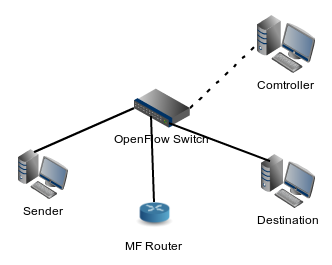
\includegraphics[width=0.3\columnwidth]{images/testcfg2.png}
\end{figure}                                                        

\tableofcontents

\pagebreak

\section{Общее описание}

\textbf{HCProbe} является реализацией библиотеки для работы с протоколом
OpenFlow на языке Haskell и предоставляет эталонную реализацию софтового
OpenFlow свича и язык для создания новых свичей, который можно использовать
для тестирования OpenFlow контроллеров.

\subsection{Перечень терминов}

\begin{description}
  \item[OpenFlow] протокол управления процессом обработки данных, передающихся
    по сети передачи данных маршрутизаторами и коммутаторами, реализующий
    технологию программно-конфигурируемой сети (SDN).
  \item[EDSL] встроенный предметно-ориентированный язык
\end{description}

\pagebreak

\section{Подсистемы}

В проекте HCProbe можно выделить сделующие подсистемы:

\begin{description}
    \item[библиотека OpenFlow] -- реализация OpenFlow протокола;
    \item[OpenFlow/Ethernet]   -- реализация генерации пакетов Ethernet-стека;
    \item[HCProbe]             -- реализация генератора сетевых пакетов и эталонной
      реализации программного свича OpenFlow;
    \item[HCProbe/EDSL]        -- предметноориентированный язык для создания контроллеров
    \item[тесты]               -- тесты создания и разбора пакетов;
    \item[примеры]             -- примеры тестов OpenFlow, разработанные с использованием
      разработанного предметно-ориентированного языка.
\end{description}


\subsection{Библиотека OpenFlow}

Библиотека OpenFlow представляет собой поддержку протокола 
OpenFlow описываемого стандартом OpenFlow spec 
v1.0\footnote{http://www.openflow.org/documents/openflow-spec-v1.0.0.pdf}
для \texttt{Haskell}. Основные модули подсистемы:

\begin{description}
    \item[Network.Openflow.Types] -- реализация структур данных, соотвествующая
        стуктурам данных OpenFlow протокола.
        \begin{itemize}
            \item инстансы \textbf{Binary.Read} для разбора структур;
            \item инстансы \textbf{Enum} для всех перечислений.
        \end{itemize}
    \item[Network.Openflow.Misc] -- дополнительные функции использующиеся в библиотеке
        \begin{itemize}
            \item функции подсчета CRC
            \item функции сериализации спецаильных типов данных
            \item функции работы с IP и MAC адресами
        \end{itemize}
    \item[Network.Openflow.Messages] -- функции серилизации и разбора сообщений OpenFlow.
\end{description}

\emph{Реализация протокола не является полной, так реализованы не все структуры из
спецификации, однако, расширение поддерживаемого протокола может выполняться по аналогии с
уже написанным кодом.}

\subsection{OpenFlow/Ethernet}

Данная подсистема предоставляет интерфейс для создания своих типов пакетов, 
которые могут быть преобразованы в стандартные сетевые пакеты. Таким образом можно создавать
специальные тестовые пакеты с определенным заданным поведением (с полями по умолчанию и т.п.).
Основные модули:

\begin{description}
  \item[Network.Openflow.Ethernet] -- реэксопортирование всех модулей, достаточно использовать только его
  \item[Network.Openflow.ARP]      -- ARP пакет
  \item[Network.Openflow.Frame]    -- сетевой фрейм (Ethernet)
  \item[Network.Openflow.IPv4]     -- IPv4 пакет
  \item[Network.Openflow.TCP]      -- TCP пакет
  \item[Network.Openflow.Types]    -- внутренние типы данных
\end{description}

\subsection{HCProbe}

HCProbe является исполняемым файлом, реализующий софтовый набор свичей, которые могут
быть взяты за эталонную реализацию программного OpenFlow свича.

Программа \texttt{hcprobe} создает указанное количество виртуальных свичей,
которые соединяются к контроллером, после чего начинают генерировать сообщения
к контроллеру, создавая полный \texttt{TCP} пакет с подствленными MAC-адресами,
относящимися к портам, используемым \texttt{HCProbe}. Каждый из свичей 
подсчитывает количество отправленных пакетов, количество полученных ответов на них,
а также количество пропущенных ответов. Полученная статистика суммируется и выводится
после выполнения программы.

Потерянным считается пакет, время ожидания ответа на который превысило указанный
интервал времени.

\subsection{EDSL}

Предметно-ориентированный язык HCProbe предназначен для создания программ свичей OpenFlow,
комбинаций этих свичей, запуска их, а также регистрации и сбора статистики по обмену
пакетами между свичами и контроллером OpenFlow.

\subsubsection{Структура программы}

Типовая программа с использованием предметно-ориентированного языка HCProbe включает
минимально 2 части:

\begin{itemize}
  \item Создание свича и задание его конафигурации;
  \item Запуска свича в соответствии с требуемой программой.
\end{itemize}

Кроме этого в большинстве случаев потребуется 3-й шаг, на котором программа дожидается
завершения работы свичей (одного или нескольких в зависимости от задачи) и получает
итоговую сводку статистики по запуску.

\subsubsection{Создание свича}

Свич создается одной из команд \lstinline!switch! или \lstinline!switchOn!. В первом случае
в качестве образца будет использован свич с конфигурацией по умолчанию, а во-втором 
переданный параметром свич. Таким образом командой \lstinline!switchOn! можно получить
копию свича, созданного ранее.

Для того, чтобы диапазоны MAC-адресов свичей не пересекались используется окружение
\lstinline!config!, в котором они и создаются:

\begin{lstlisting}
    sw <- config $ switch <switchIP> $ do ..
\end{lstlisting}%$

\subsubsection{Настройка возможностей свича}

Настройки свича проводятся в окружении \lstinline!features!, в котором можно задать
параметры свича.

\begin{lstlisting}
    switch <switchIP> $ do
      features $ do
        ..
\end{lstlisting}

К настройкам относятся, например порты, добавляемые командой \lstinline!addPort!.

Команда \lstinline!addMACs! добавляет список MAC-адресов к свичу, при этом они разделяются
поровну между портами этого свича.

\lstinline!clearMACs! удаляет все MAC-адреса, добавленные к свичу.


\subsubsection{Запуск свича}

Свич может быть запущен в 2 вариантах:

\begin{itemize}
  \item если для задачи подходит стандартная реализация логики свича, то запускать
    его следует при помощи функции \lstinline!runSwitch!;
  \item чаще требуется задание какой-то конкретной логики поведения свича, которая
    может быть задана при выполнении функции \lstinline!withSwitch!.
\end{itemize}


\subsubsection{Выполнение программы}
Полсле запуска свича (при помощи \lstinline!withSwitch!) он начианет выполнять
переданную ему программу, данный блок является обычным блоком haskell кода,
который может взаимодействовать со свичем, используя созданные для этого команды,
среди которых есть следующие:

\begin{description}
  \item[hangOn] -- ожидать вечно, может быть полезно в случае если нужно тестировать
свич.

  \item[waitForType] -- ожидание определенного типа сообщения: выполнение прогаммы
будет прервано то тех пор, пока не придет сообщение указанного типа, возвращает 
полученное сообщение.

  \item[waitForBID] -- ожидание сообщения с указанным значением \lstinline!buffer id!.
Возвращшает полученное сообщение.

\end{description}

Для генерации сообщений желательно, чтобы используемые номера транзакций и буфферов 
не пересекались, для этого служат команды \lstinline!nextBID! и \lstinline!nextTID!.

Для отправки сообщений могут быть использованы следующие команды:

\begin{description}

  \item[send] -- отправка произвольного пакета OpenFlow контроллеру;

  \item[sendOFPacketIn] -- отправка пакета типа \lstinline!OFPT_PACKET_IN!;

  \item[sendARPGreeting] -- отправка контроллеру пакета \lstinline!OFPT_PACKET_IN!
    с ответом ARP внутри (может понадобиться для случая, когда нам нужно проверить
    ситуацию в которой контроллер должен знать MAC-адрес или адреса);

  \item[statsSend/statsSendOFPacketIn] -- варианты \lstinline!send! и
    \lstinline!sendOFPacketIn! со сбором статистики при отсылке пакетов.

\end{description}

\subsubsection{Сбор статистики}

Текущая реализация поддерживает сбор следующих параметров статистики:

\begin{itemize}
  \item число отосланных пакетов;
  \item число пакетов с ответами от контроллера;
  \item число пакетов без ответов от контроллера (факт отсутствия ответа обозначается,
    когда очередь ожидания ответов становится переполненной);
  \item времена ответов от сервера (вычисляется как разница времени отправки пакета
    и получения ответа на него).
\end{itemize}

Собственно, само использование статистики подразумевает следующие шаги:

\begin{itemize}
  \item вызов \lstinline!initPacketStats! для создания cущности \lstinline!StatsEntity!,
    в которой будут храниться данные статистики;
  \item регистрация обработчика статистики для свича при помощи 
    \lstinline!setSilentStatsHandler! или \lstinline!setStatsHandler stEnt ...!,
    второй вариант предназначен для того, чтобы, к примеру, выводить в консоль или
    файл факты регистрации ответа на отсылку пакета контролллеру;
  \item отсылка пакета контроллеру при помощи команд \lstinline!statsSend! или
    \lstinline!statsSendOFPacketIn!;
  \item получение сводной статистики по контроллерам при помощи команды
    \lstinline!assembleStats!.
\end{itemize}

\subsubsection{Изменение ответов контроллеру по умолчанию}

Для того, чтобы изменить поведение свича на сообщения контроллера (например, для
проверки реакции контроллера на ошибочное поведение свича, потерю пакетов и т.п.)
можно использовать команду \lstinline!setUserHandler!, которая позволяет задать
необходимую по задаче реакцию.

\emph{В текущей реализации статистика работает также через \lstinline!setUseHandler!,
поэтому одновременно эти два механизма пока использовать не рекомендуется.}

\section{Приложения}

\subsection{Параллельное выполнение свичей}

Для параллельного запуска нескольких свичей и контроля за временем исполнения
используется библиотека asyc\footnote{http://hackage.haskell.org/package/async}

Самым простым приёмом может быть ограничение выполнения запуска свича по времени:

\begin{lstlisting}
import Control.Concurrent (threadDelay)
import Control.Concurrent.Async (race_)

...
race_ action1 (threadDelay 1000000)
\end{lstlisting}

Здесь, подразумевается что action1 содержит запуск нужного свича, таким образом
выполнение этой строки завершится или по завершении программы свича (если она
отличается от программы по-умолчанию и конечна) или по истечении одной секунды.

Если же запускается одновременно несколько свичей, то типовым решением будет
запуск каждого из них в отдельном потоке (при помощи \lstinline!async!) и ожидание
их окончания (или истечения интервала времени, если это необходимо).

Схематически это будет выглядеть примерно следующим образом:

\begin{lstlisting}
  a1 <- async $ withSwitch sw1 ...
  ...
  aN <- async $ withSwitch swN ...
  mapM_ waitCatch [a1,....,aN]
\end{lstlisting}

Если выполнение программы стоит приостановить при появлении ошибки в любом из
свичей, то \lstinline!waitCatch! следует заменить на \lstinline!wait!.

Конечно же вместо \lstinline!withSwitch! может стоять \lstinline!runSwitch!
в зависимости от задачи.

\subsection{Примеры программ}

\subsubsection{Простейший свич}

Это один из простейших примеров, тут задаётся 2 свича,
выводится в консоль конфигурация второго и запускается
первый с программой по умолчанию с ограничением работы
в 3 секунды.

\begin{lstlisting}
{-# LANGUAGE OverloadedStrings #-}
module Main
  where

import Control.Concurrent (threadDelay)
import Control.Concurrent.Async (race_) -- EDSL for asynchronous actions
import Data.Bits                        -- for IP creation
import HCProbe.EDSL

main = do 
    let ip = 15 .|. (0x10 `shiftL` 24)
    (sw1,sw2) <- config $ do
      sw1 <- switch ip $ do
            features $ do
                {- replicateM 48 $ --uncomment to create 48 ports -}
                addPort [] [] [OFPPF_1GB_FD, OFPPF_COPPER] def
                addPort [] [] [OFPPF_1GB_FD, OFPPF_COPPER] def
            addMACs [1..450]
      sw2 <- switchOn sw1 $ do
                clearMACs 
                addMACs [400..500]
      return (sw1,sw2)
    print sw2
    race_ (runSwitch sw1 "localhost" 6633) (threadDelay 3000000)
\end{lstlisting}

% Идеи, что еще можно сделать с eDSL
% 1. Измениение длины пакета. Было бы здорово, если можно было бы напрямую задать значение этого поля в OF Header'е. А не влиять на нее косвенно, задавая только длину заголовка.
% 2. Генерация кривых кадров внутрь PacketIn. Также, чтобы можно было менять поля (хочу положить в Ethernet кадр IP пакет, а в заголовке написать, что это ARP), прям при создании сообщения. Сейчас для этого надо делать instance EthernetFrame.
% 3. Вообще, можно для всех типов сообщений сделать генераторы по типу putPacketIn, чтобы не приходилось этого делать через putOFData/putRaw
% 4. Очень нетривиально для человека, который не знает haskell, сделать генерацию неправильных ASCII-строк:) Но, я думаю, можно не считать это распространенным юзкейсом.
% 5. Не знаю, какую-то юзер-френдли статистику. Пока без примеров непонятно, как ее делать.
% 6. Нужен пример с несколькими свичами (с одинковой программой для каждого и с разными)

\end{document}
